After the compact ablation had selected Model 03 as the strongest model family, the
winning design was trained and locked again as the final report model package. The
reason is that the ablation suite is model-selection evidence, while the downstream
pipeline needs one reproducible checkpoint tied to the final data contract. The final
package, \texttt{full\_gode\_havnebilleder\_tau06\_final\_2026\_06\_05}, therefore
uses the same BCE + Dice and GroupNorm design, but is tied to the final 1,143
image-mask pairs, the 914/114/115 chronological split, LA/LB represented under
\texttt{long\_beach}, 2nd/98th percentile image normalization, geometric
augmentation, no photometric augmentation, and the checkpoint used in the downstream
pipeline.

The selected checkpoint is epoch 96. This is the epoch with the lowest validation
loss in the final training log, with validation loss 0.3834 and validation Dice
0.6707 at \(\tau=0.4\). The final supervised report evaluation at the same threshold
gives validation Dice 0.6707 and test Dice 0.6323 before ROI filtering. With ROI10
post-processing, the test Dice is 0.6353. The model should therefore be read as the
final retrained Model 03 package, not only as the earlier ablation candidate.

\begin{figure}[H]
    \centering
    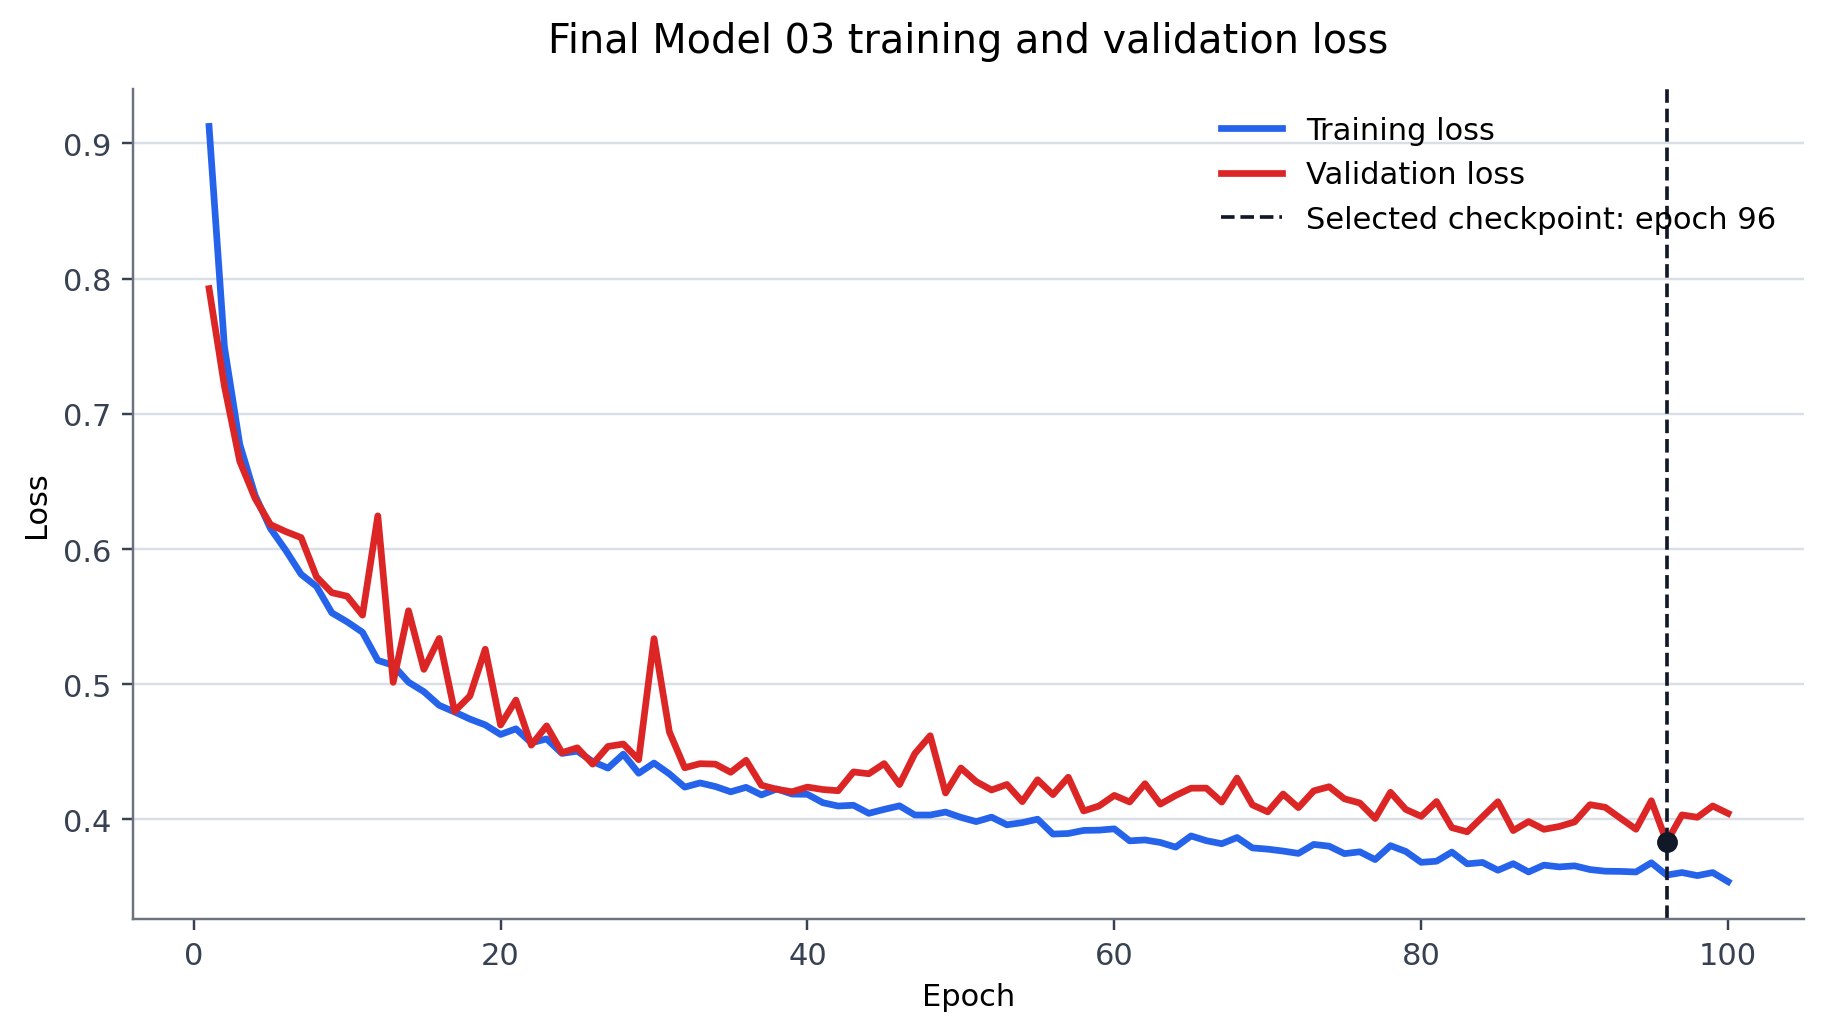
\includegraphics[width=0.92\linewidth]{FinalFigures/final_model03_train_loss_vs_val_loss.png}
    \caption{\textbf{Final Model 03 training and validation loss.} The curves show the retrained and locked report model package after Model 03 had been selected in the compact ablation suite. The dashed line marks the selected checkpoint at epoch 96, where validation loss reaches its minimum.}
    \label{fig:final_model03_train_val_loss}
\end{figure}

\begin{figure}[H]
    \centering
    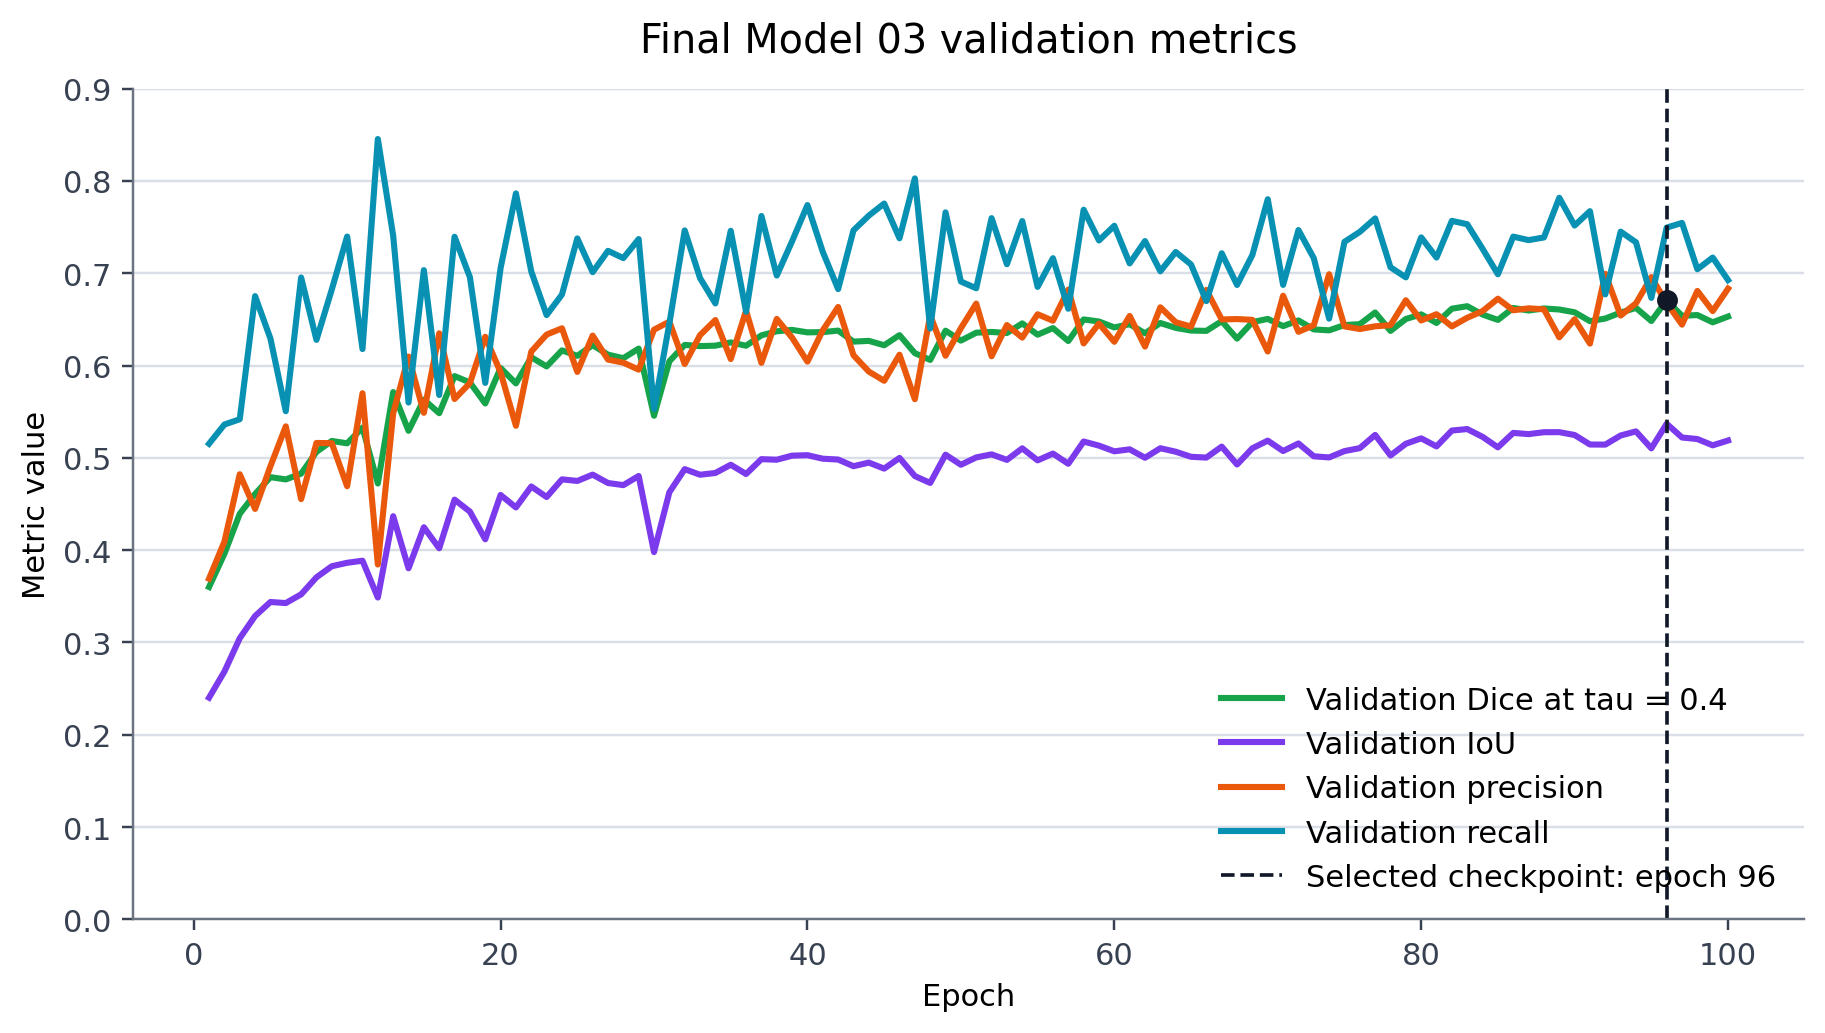
\includegraphics[width=0.92\linewidth]{FinalFigures/final_model03_validation_metrics_over_epochs.png}
    \caption{\textbf{Final Model 03 validation metrics.} The curves show the validation metrics saved during training of the final report model package. Validation Dice at \(\tau=0.4\) peaks at epoch 96, matching the selected checkpoint used for final supervised evaluation and downstream inference.}
    \label{fig:final_model03_validation_metrics}
\end{figure}
